\subsection{Output files}
After having run an optical simulation an overview of the results can be seen in the optical simulation window (Figure \ref{fig:transfermatrix0}) as described above. However more in depth information can be obtained from the \emph{Output} tab of the main window as shown in Figure \ref{fig:transfer_matrix_optical_output}.

\begin{figure}[H]
\centering
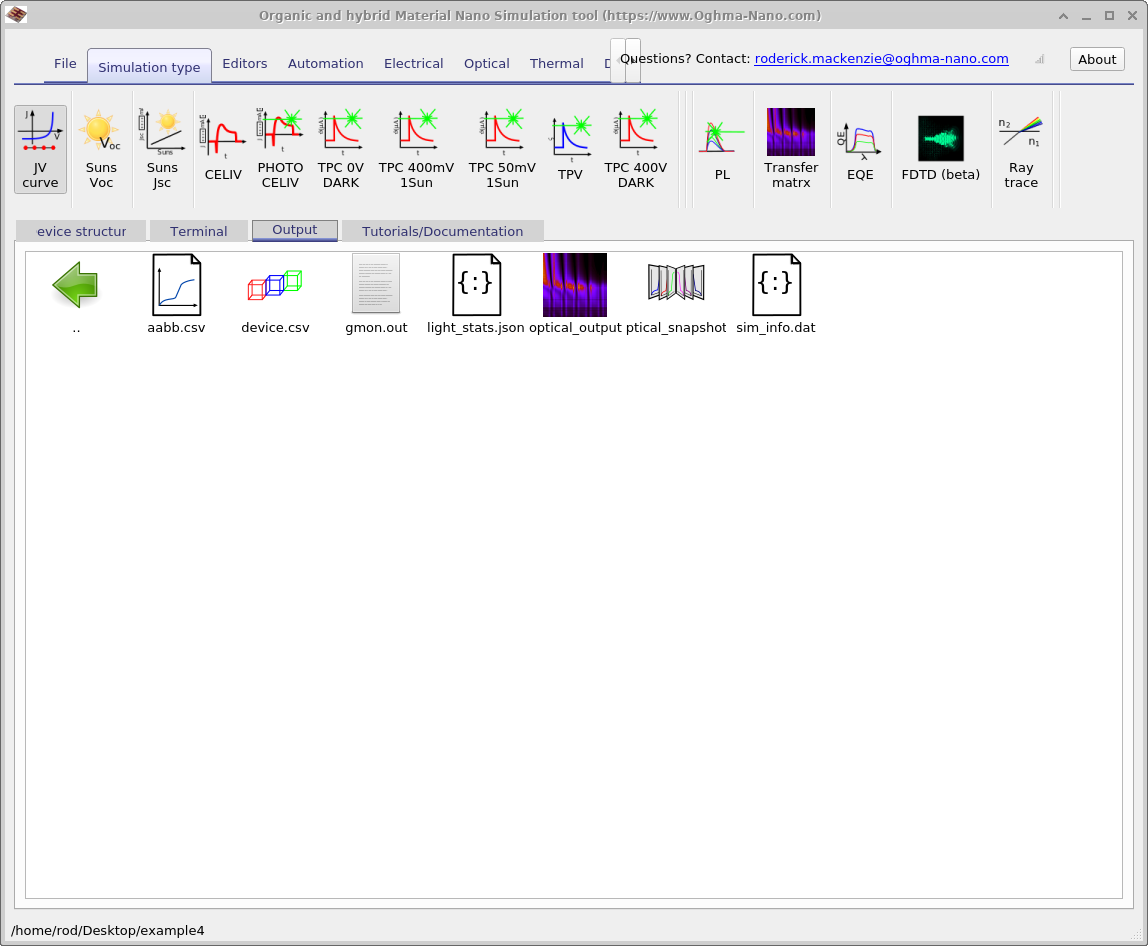
\includegraphics[height=0.6\textwidth,width=0.7\textwidth]{./images/transfer_matrix/optical_output.png}
\caption{The output tab shows the output from the transfer matrix simulation. Usually the optical\_output and optical\_snapshots files are only generated when the optical simulation is run directly and not as part of another simulation.}
\label{fig:transfer_matrix_optical_output}
\end{figure}

In Figure \ref{fig:transfer_matrix_optical_output} you can see two icons one called \emph{Optical output} and the other called \emph{optical\_snapshots} (in the figure it reads "ptica\_output" due to the text being hidden). If you double click on \emph{Optical output} it will bring up figure \ref{fig:transfermatrix0}. If you double click on \emph{optical\_snapshots} it will bring up Figure \ref{fig:transfer_matrix_optical_snapshots}. The optical snapshot window allows the user to view photon density, absorbed photons and electric field of the light. The information is displayed per wavelength so a detailed overview of device performance can be gained.


\begin{figure}[H]
\centering
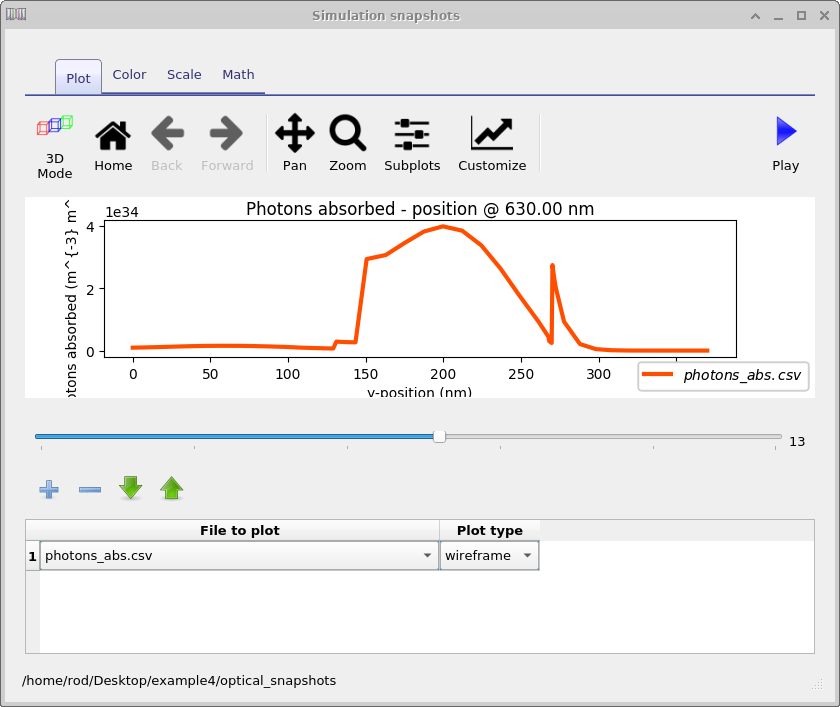
\includegraphics[height=0.6\textwidth,width=0.7\textwidth]{./images/transfer_matrix/optical_snapshots.png}
\caption{The optical snapshots window. This allows the user to view, Electric }
\label{fig:transfer_matrix_optical_snapshots}
\end{figure}

\subsubsection{The optical\_snapshots directory in depth}
The optical\_snapshots folder was described above and when accessed through the graphical interface allows the user to access photon density, absorbed photons and electric field of the light as a function of wavelength. However, it is simply a normal directory and the user can access it through a file explorer. If you open the directory using a tool such as windows explorer you will see something comparable to what is shown on the left of Figure \ref{fig:optical_snapshots_dir}. You can see folders numbered from 0 to 12 each folder represents a simulated wavelength. If you open a directory, say number 0, you will be presented with the files shown in the right hand of figure \ref{fig:optical_snapshots_dir}. These files contain the following information:

\begin{table}[H]
\begin{center}
\begin{tabular}{ |c|l|c| } 
 \hline
	File name 			& 	Description  \\ 
 \hline
	$alpha.csv$			&	y-position v.s. absorption @ given wavelength \\ 
	$data.json$			&	json file containing wavelength value \\ 
	$En.csv$ 			&	y-position (m) v.s. Electric field with -ve component (V/m)  @ given wavelength \\ 
	$Ep.csv$ 			&	y-position (m) v.s. Electric field with +ve component (V/m) @ given wavelength \\ 
	$G.csv$ 			&	y-position (m) v.s. Generation rate ($m^{-3} s^{-1}$)\\ 
	$n.csv$ 			&	y-position (m) v.s. Real part of the refractive index n (au) @ given wavelength\\ 
	$photons.csv$ 		&	y-position (m) v.s. photon density ($m^{-3}$) @ given wavelength \\ 
	$photons\_abs.csv$ 	&	y-position (m) v.s. photons absorbed ($m^{-3} s^{-1}$) @ given wavelength\\ 
 \hline
\end{tabular}
\caption{Files produced by the JV simulation}
\label{tab:jv_output}
\end{center}
\end{table}


\begin{figure}[H]
\centering
\begin{tabular}{ c c }

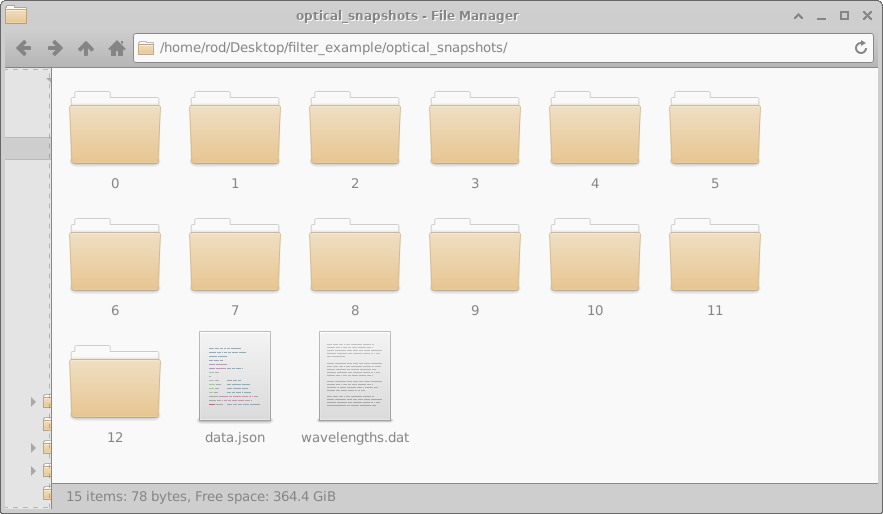
\includegraphics[width=0.5\textwidth,height=0.35\textwidth]{./images/transfer_matrix/snapshots_main_dir.png}

&
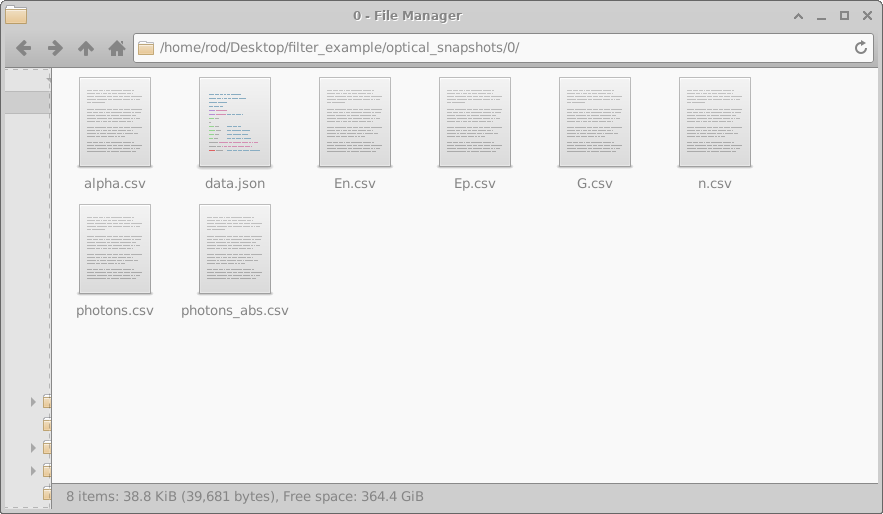
\includegraphics[width=0.5\textwidth,height=0.35\textwidth]{./images/transfer_matrix/snapshots_sub_dir.png}

\\
\end{tabular}
\caption{Various views of the optical simulation window}
\label{fig:optical_snapshots_dir}
\end{figure}

These files are simply plain text, if you open one it will look like \ref{fig:transfer_matrix_file_example}. The first line of this file contains some information about the content of the file to help with plotting. The second line tells the user what the x and y axis contain then the following lines contain the data.

\begin{figure}[H]
\centering
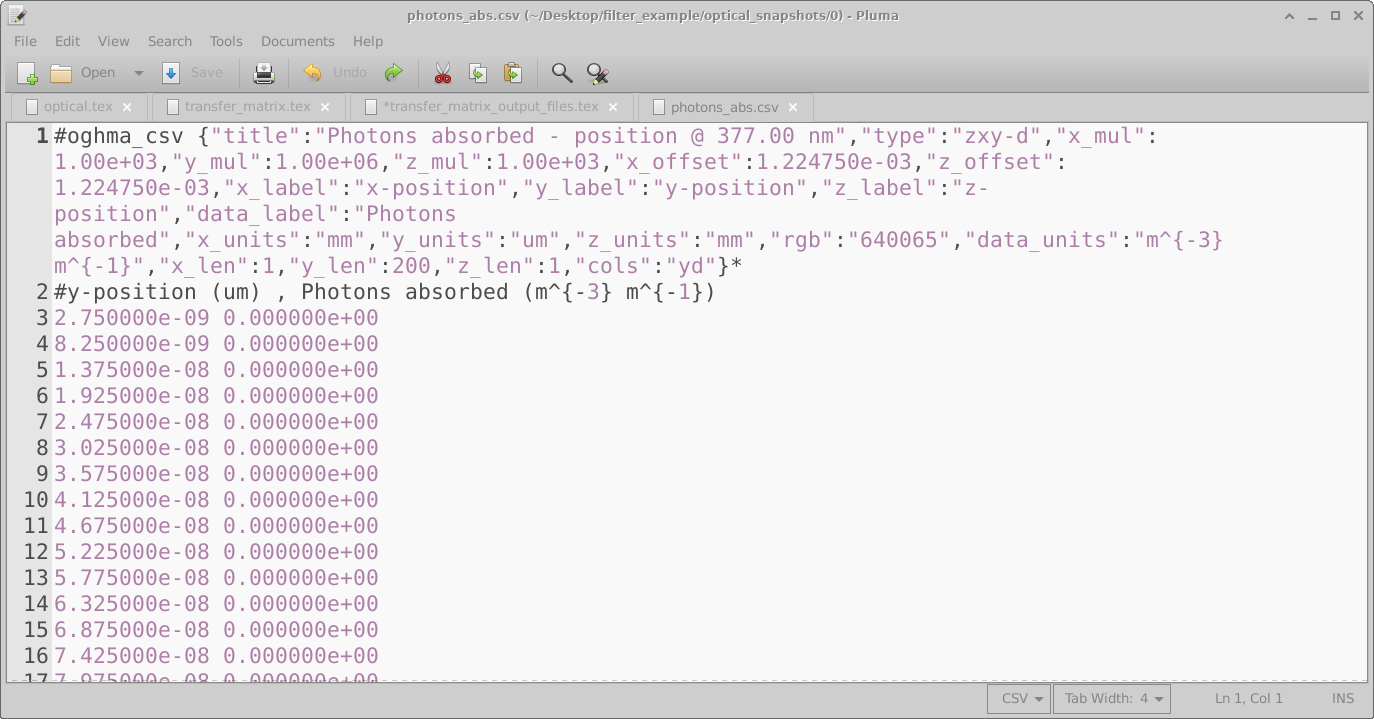
\includegraphics[height=0.5\textwidth,width=0.7\textwidth]{./images/transfer_matrix/snapshots_file_example.png}
\caption{The content of photons\_abs.csv.}
\label{fig:transfer_matrix_file_example}
\end{figure}

\subsubsection{The optical\_output folder in depth}
While the optical\_snapshots directory allows data to be plotted per simulated wavelength, the optical\_output gives 2D maps of wavelength v.s. position for various simulation parameters. The content of the directory is shown in figure \ref{fig:optical_output_directory}.

\begin{figure}[H]
\centering
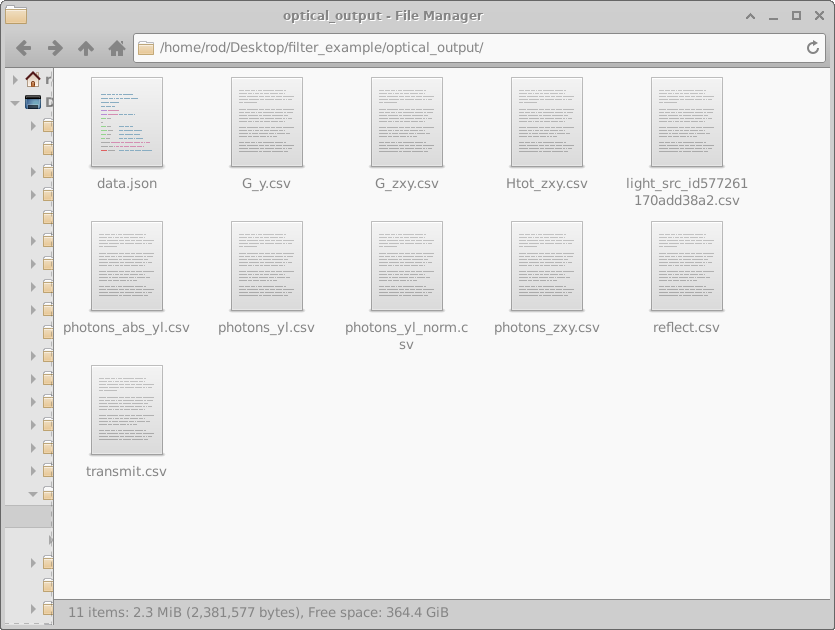
\includegraphics[height=0.5\textwidth,width=0.7\textwidth]{./images/transfer_matrix/optical_output_dir.png}
\caption{The content of optical\_output directory}
\label{fig:optical_output_directory}
\end{figure}

The files shown in Figure \ref{fig:optical_output_directory} are described in table \ref{tab:optical_output_files}.

\begin{table}[H]
\begin{center}
\begin{tabular}{ |c|l|c| } 
 \hline
	File name 				& 	Description  & Plot type\\ 
 \hline
	data.json				&	Miscellaneous simulation information in json format			&	1D \\
 	G\_y.csv				&	y-position (m) v.s. Charge generation rate ($m^{-3} s^{-1}$)&	2D \\
	G\_zxy.csv				&	zxy-position (m) v.s. Charge generation rate ($m^{-3} s^{-1}$)	&	2D \\
 	Htot\_zxy.csv			&	zxy-position (m) v.s. Optical heat generation ($W m^{-3}$)	&	2D \\
 	light\_src\_id\_xxx.csv	&	wavelength (m) v.s. Light intensity from source ($W/m$)		&	2D \\
 	photons\_abs\_yl.csv	&	wavelength (m) v.s. y-position (m) v.s. photons absorbed ($m^{-3} s^{-1}$)	&	2D \\
 	photons\_yl.csv			&	wavelength (m) v.s. y-position (m) v.s. Photon density ($m^{-3} s^{-1}$)&	2D\\
 	photons\_yl\_norm.csv	&	wavelength (m) v.s. y-position (m) v.s. Normalized photons (au)&	2D \\
 	reflect.csv				&	wavelength (m) v.s. Light reflected from the stack 	&	1D  \\
 	transmit.csv			&	wavelength (m) v.s. Transmitted though the stack	&	1D  \\
 \hline
\end{tabular}
\caption{Files produced by the JV simulation}
\label{tab:optical_output_files}
\end{center}
\end{table}

\newpage


